\chapter{The Case\label{case}}

\section{Architecture}
Before refactoring the studied application was build using monolith architecture following a three tier pattern containing frontend, backend and database.
The backend was written using Node.js version v14.19.1 that uses V8 engine version \textit{8.4.371.23-node.85}.
It contains multiple components each with its own purpose.
One of the components were refactored out of the monolith application into the independent service.

The independent service contained an application interface to allow communication to the component and the component itself.
The independent service was build using Node.js with version v14.18.3 that uses V8 engine version \textit{8.4.371.23-node.85}.
The architecture before and after refactoring can be seen in figures \ref{figure:architecture:monolith} and \ref{figure:architecture:independent_service}.

\begin{table}[h!]
    \begin{tabular}{|c c|} 
         \hline
         Node.js version & V8 version \\ [0.5ex] 
         \hline
         14.18.3 & 8.4.371.23-node.85  \\ 
         \hline
          14.19.1 & 8.4.371.23-node.85  \\ 
         \hline
    \end{tabular}
    \caption{Node.js versions an the V8 engine they use.}
    \label{table:node:versionsWithV8}
\end{table}

\begin{figure}
    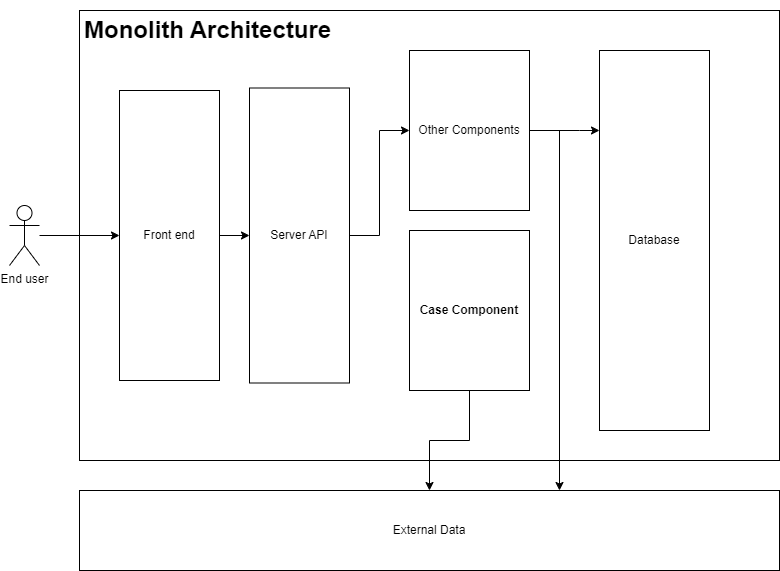
\includegraphics[width=\textwidth]{images/monolith_architecture.png}
    \caption{Architectural overview of the application before refactoring.}
    \label{figure:architecture:monolith}
\end{figure}
\begin{figure}
    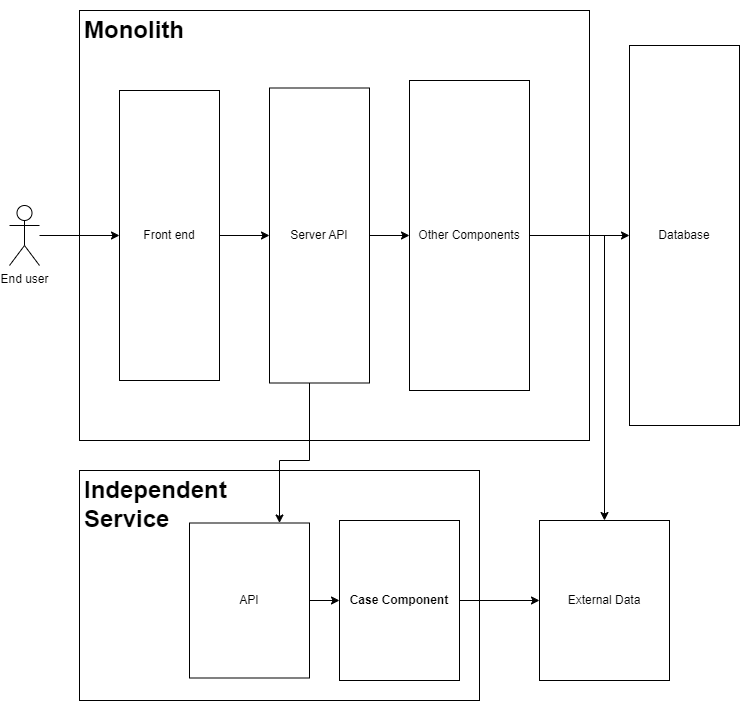
\includegraphics[width=\textwidth]{images/independent_service_arcitecture.png}
    \caption{Architectural overview of the application after refactoring the component into independent service.}
    \label{figure:architecture:independent_service}
\end{figure}

Both environments, the monolith and the independent service, were running in linux server provided by amazon web services.
The hardware specs differed for both environment.
The monolith had 64GB RAM with 8 vCPU of computing power while the independent service had 4GB of RAM with 1 vCPU of computing power available.
The use of production environment didn't allow to utilize same resources for both environments.

\begin{table}[h!]
    \begin{tabular}{|c|c|c|c|c|} 
        \hline
        Environment
        & RAM (GB)
        & Core (vCPU)
        & Node.js version
        & V8 version
        \\ 
        \hline
        Monolith
        & 64GB
        & 8
        & v14.19.1
        & 8.4.371.23-node.85
        \\
        \hline
        Independent service
        & 8GB
        & 1
        & 14.18.3
        & 8.4.371.23-node.85
        \\
        \hline
    \end{tabular}    
    \caption{Hardware specification.}
    \label{represented:harware:specs}
\end{table}

\section{Overview of the Component}
The component is written using javascript and it is run in node.js runtime environment.
While the component is running it performs cycles that consist of two or four tasks.
Completing all task is called a full cycle.
When a cycle is finished a new one is started and the cycles run until the process is manually stopped.

Full cycle contains four tasks.
Each task is represented by its own module and each module is run sequentially one after the other
all of the modules response time is critical to the system.
Any error interrupts the cycle resulting in a halt of the process.
\begin{itemize}
    \item
    \textbf{Module A} is the first module in the cycle.
    It is always called when the cycles are running.
    
    \item
    \textbf{Module B} is the second module in the cycle.
    It runs after \textbf{module A}.
    
    \item
    \textbf{Module C} is the third module in the cycle.
    It runs after \textbf{module B} only when the response from \textbf{module A} requires it to run.
    Otherwise rest of the modules in the cycle are skipped and the cycle restarts from \textbf{module A}.

    \item
    \textbf{Module D} is the last module in the cycle.
    After it is finished the cycle is restarted from \textbf{module A}.
\end{itemize}

Modules A, C and D are dependent on external data.
Module D is dependent on module C and module C is dependent on module A.
All modules are dependent in input parameters in a way that user can determine when the process is halted and continued.
Error at any point of the cycle ends the process requiring manual restart of the cycle from the user.
The dependencies of the modules can be seen in figure \ref{figure:module:relation}.
The flowchart of the modules are shown in figure \ref{figure:module:flow}.

\begin{figure}
    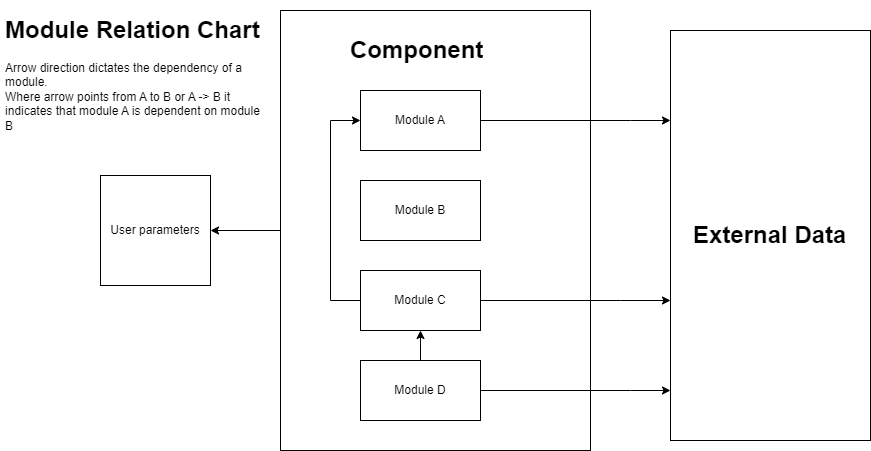
\includegraphics[width=\textwidth]{images/modules_relation_uml.png}
    \caption{Components modules and their dependencies.}
    \label{figure:module:relation}
\end{figure}


\begin{figure}
    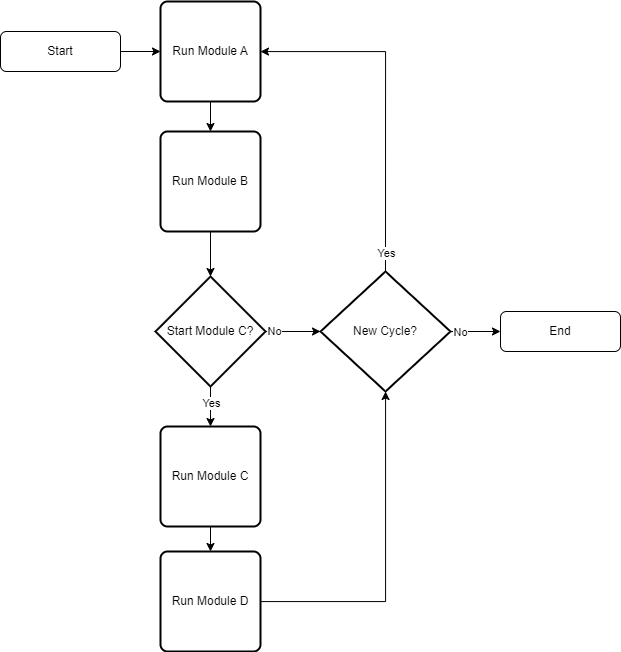
\includegraphics[width=\textwidth]{images/module_flow_chart.png}
    \caption{Modules flowchart. Modules are run inside the studied component.}
    \label{figure:module:flow}
\end{figure}

When any of the modules fails to perform its task an error is raised and the cycle is interrupted.
When modules are running without errors the modules A and B are always performed. 
The modules C and D are run only when the data from \textbf{module A} requires them to run.
Each module waits for the response of external calls before continuing their process.

\section{Performance of the Case}
This research studies performance of a server side JavaScript software component.
Performance is defined as the time the component takes to processing its blocking events.
All non blocking calls from the component are timed and excluded from the performance review in order to capture the response time of all blocking events in the component.
The component performance is measured when it is a part of a monolith application and when it is refactored into its own service.
The component is not modified between environments.
Its performance is critical to the system.
